\documentclass[../mciAusarbeitung.tex]{subfiles}

\usepackage[utf8]{inputenc}
\usepackage[T1]{fontenc}
\usepackage{lmodern}
\usepackage[german]{babel}
\usepackage[fixlanguage]{babelbib}
\selectbiblanguage{german}
\usepackage{amssymb}
\usepackage{graphicx}
\usepackage{url}
\usepackage{float}

\title{Fachpraktikum MCI (01513) - WS 2021/22}
\author{Gruppe 2\\
	Sabine Hopf}
\date{\today}

\begin{document}
	Wie schon im Abschnitt 1.4 beschrieben, kann man unter dem Menüpunkt ,,Beispiele'' die vordefinierten Konfigurationen für die exemplarischen Beispiele der kooperativen Ausgaben abrufen.\\
	Die Klasse \textit{ConfigurationIOHelper} im Package \textit{de.fernunihagen.mci.group2.coopalgoart.impl.config} erzeugt eine \textit{json}-Datei \textit{(JavaScript Object Notation)}. Diese dient dazu die Konfiguration abzulegen.\\
	Um z. B. die Parameter eines Bildes der unten gezeigten Ergebnisse aller Generatoren zu erhalten, öffnet man den Menüpunkt ,,Beispiele'' und wählt dann das Untermenü ,,Kooperation'' und ,,Ausarbeitung''. Hier kann man dann eines der hier vorgestellten Beispiele auswählen. Nach Klick auf das gewünschte Beispiel, wechselt die GUI zur Ansicht der geforderten Konfiguration. Hier sind alle Parameter schon so abgespeichert, wie sie in unseren Beispielen verwendet wurden. Nach einem Klick unten auf ,,Testlauf'' erhält man nach Ablauf der eingestellten Iterationen, das von uns als exemplarisches Ergebnis eingestellte Bild.

	\subsection{Kooperative Ergebnisse aller Generatoren}
	Nachstehend werden die Ergebnisse beschrieben und gezeigt, die aus der Kooperation von Generatoren verschiedener Gruppenmitglieder entstanden sind.\\	
	\\
	Das erste Beispiel unten ,,Buntes Treiben'' verbindet die Generatoren ,,perlinNoise'' von G. Rißland, ,,GOL'' von C. Camier, ,,LSystemBuilder'' von B. Winzen und ,,Evolution'' von S. Hopf miteinander. Dabei beeinflussen die Parameter des ,,perlinNoise'' die Startaufstellung des ,,GOL'', diese Parameter manipulieren die Position, Größe und Farbe des ,,Sterns'' des ,,LSystemBuilder''. Dessen Position wiederum wirkt auf die Position des Ziels der ,,Evolution'' ein.\\
	Es wurde der Koopmode ,,Übereinander'' gewählt. \\
		\begin{figure}[H]
			\centering
			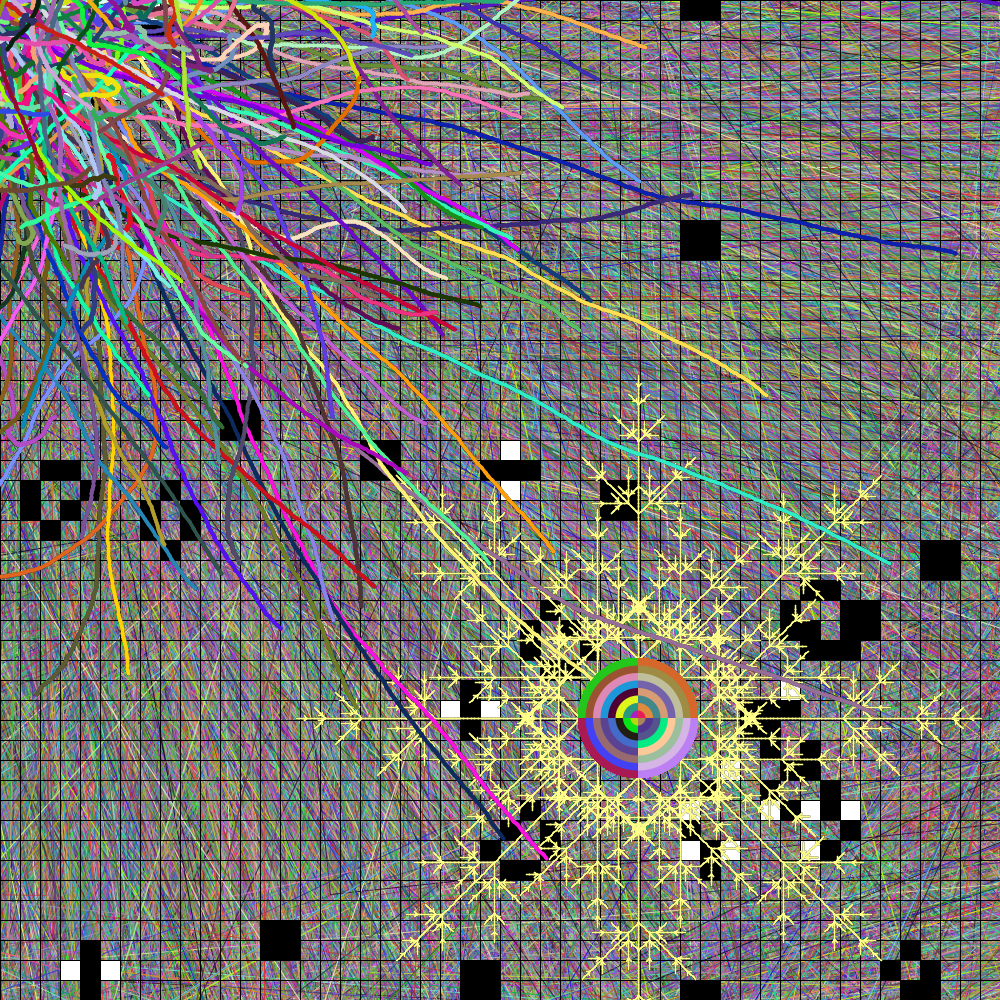
\includegraphics[width=0.8\linewidth]{img/buntesTreiben.png}
			\caption[Buntes Treiben]{Kooperation perlinNoise, GOL, LSystemBuilder, Evolution (eigene Darstellung)\\
			Bildgenerierung:,,Menübar/Beispiele/Kooperation/Ausarbeitung/Buntes Treiben''}
		\end{figure}
	\noindent Das zweite Beispiel unten ,,Rosa Welt'' verbindet die Generatoren ,,Cautomate'' von G. Rißland, ,,GOL'' von C. Camier, ,,Lsystem'' von S. Hopf und ,,Swarm'' von B. Winzen miteinander. Dabei beeinflussen die Parameter des ,,Cautomate'' die Startaufstellung des ,,GOL'', diese Parameter wirken auf die Winkel, die Länge der Zweige und die Startposition der Bäume > 1 ein. Der ,,Swarm'' wird durch den Kooperationspunkt des Baumes angezogen, da die Option ,,Kooperation via Anziehung'' ausgewählt wurde. Auch hier wurde der Koopmode ,,Übereinander'' gewählt.\\
		\begin{figure}[H]
			\centering
			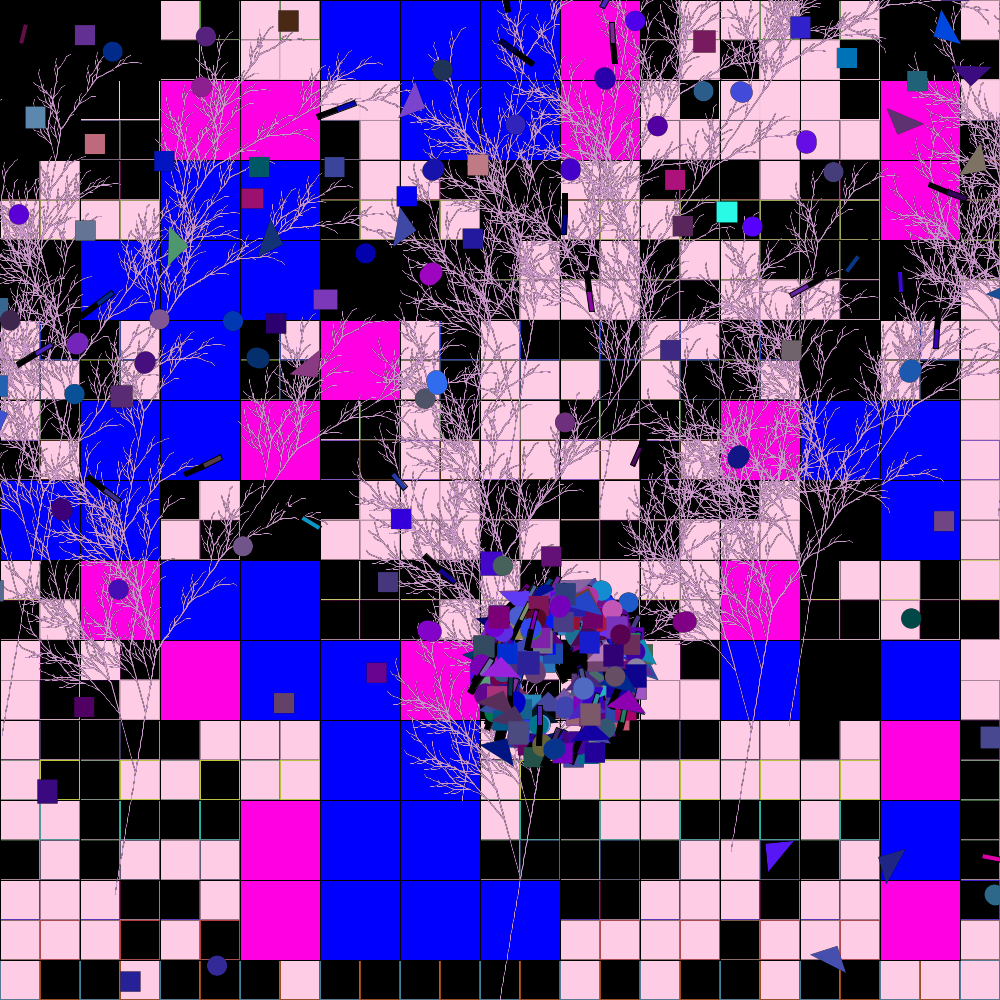
\includegraphics[width=0.8\linewidth]{img/rosaWelt.png}
			\caption[Rosa Welt]{Kooperation Cautomate, GOL, LSystem, Swarm (eigene Darstellung)\\
			Bildgenerierung:,,Menübar/Beispiele/Kooperation/Ausarbeitung/Rosa Welt''}
		\end{figure}
	\noindent Das dritte Beispiel unten verbindet die Generatoren sowohl übereinander als auch nebeneinander, durch den Koopmode ,,Geteilte Bereiche 2x2''.\\
	 Im Einzelnen sieht man hier im linken oberen Quadrat ,,LSystemBuilder'' von B.Winzen, ,,LSystem'' von C. Camier und ,,LSystem'' von S. Hopf. Im rechten oberen Quadrat findet man ,,Swarm'' von B. Winzen, ,,Swarm'' von S. Hopf und ,,flocking'' von G. Rißland. Im linken unteren Quadrat kann man ,,GOL'' von C. Camier und ,,Cautomate'' von G. Rißland ausmachen. Im rechten unteren Quadrat entdeckt man schließlich ,,perlinNoise'' von G. Rißland und ,,Evolution'' von S. Hopf.\\
	Die Parameter der einzelnen Generatoren werden aber weiterhin in der Reihenfolge ihres Auftretens beeinflusst, das bedeutet, der ,,LSystemBuilder'' links oben beeinflusst den ,,Swarm'' rechts oben, dieser wieder ,,perlinNoise'' links unten usw.\\
		\begin{figure}[H]
			\centering
			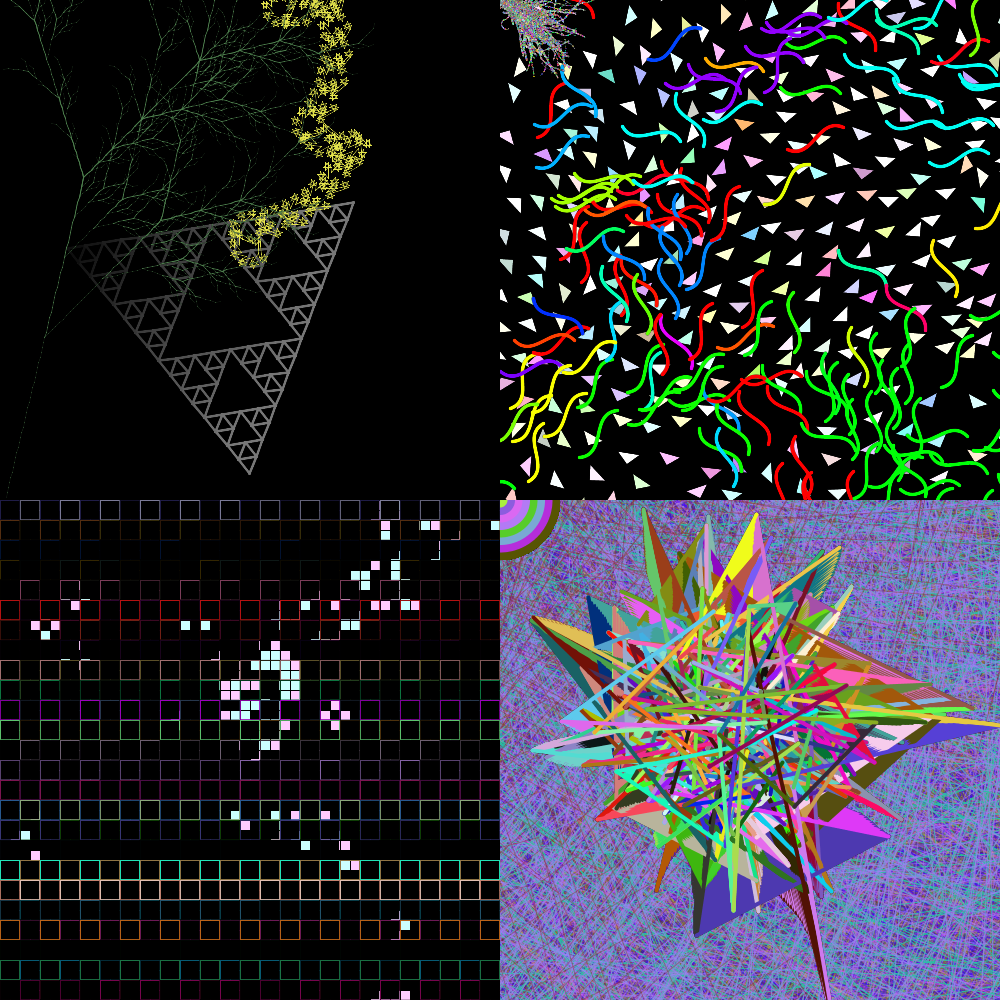
\includegraphics[width=\linewidth]{img/allesInEinem.png}
			\caption[Alles in einem]{Kooperation LSystemBuilder, Swarm, GOL, perlinNoise, LSystem, Swarm, Cautomate, Evolution, LSystem, flocking (eigene Darstellung)\\
			Bildgenerierung:,,Menübar/Beispiele/Kooperation/Ausarbeitung/Alles in einem''}
		\end{figure}
	
\end{document}